%% dp: This title is pretty vague.  
%\section{Addressing the Combination of \java{} and \sgx{}}
\section{\java{} Support for Partitioning into \sgx{}}
\label{sec:concept}

This section explains the support \systemname{} adds to \java{}
for partitioning applications into \sgx{} enclaves.
%support in addresses the challenges
%in partitioning \java{} applications on 

\subsection{Cleanly partitioning classes and objects}
\label{sec:concept:partition}

%To address the partition challenge in a managed language like \java{},
%\systemname{} diminishes the need for developers
%to scrutinize the whole code base
%and identify the fine line of isolating trusted and untrusted classes. 

\systemname{} includes Shredder to automatically partition \java{} applications on \sgx{},
requiring  minimal developer effort.
Figure~\ref{fig:builder} shows the workflow of a developer using the \systemname{} Shredder tool.
The developer selects the application's main class, either as a JAR or class files
and the classpath of the library.
The developer also specifies the list of
entry classes that should be in the enclave and export an interface to the code 
outside of the enclave.
%% When developers use the tool to partition their applications, they provide
%% the application package, either in JAR or classes,
%% the class paths of the depended libraries,
%% and a list of {\em entry classes} as the initial entry points of the enclave.
The Shredder then
identifies all classes that the entry classes depend upon,
until the transitive closure of these dependencies converges.
%performs {\bf dependency tracking} starting at the entry classes,
%until all the depended classes eventually converge.
%% dp: this feels out of place here; maybe put it at the beginning of the section?
%Afterward, \systemname{} packages the classes, with additional steps of augmentation, instrumentation, and signing, purpose of which is explain in \S\ref{sec:concept:loading} and \ref{sec:concept:accessing}.

\begin{figure}[t!]
\centering
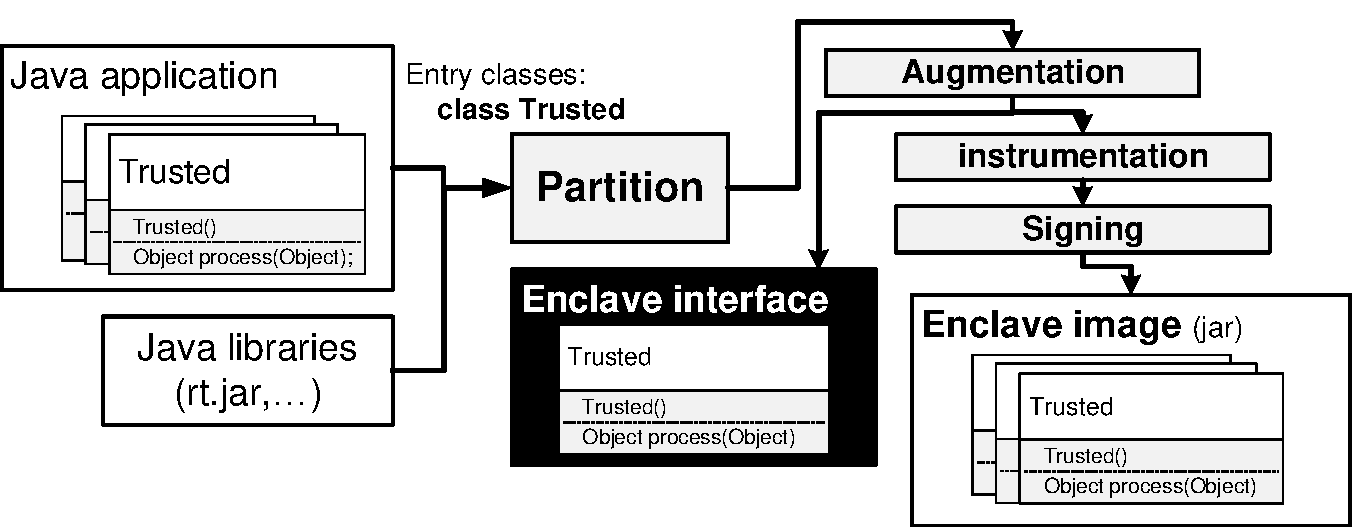
\includegraphics[width=\linewidth]{civet/figures/building-tool.pdf}
\caption{\systemname{} design-time tool, for partitioning, packaging, augmentation, instrumentation, and signing.
\systemname{} partitions the \java{} application based on the entry classes
specified by the developers (classes {\tt Trusted}).
The Shredder tool recursively pulls all required supporting classes into the 
package to run in the enclave.
%from all the class paths.
%Only the minimum necessary classes are kept for the enclave,
The Shredder tool creates an enclave JAR file after augmentation,
instrumentation, and signing.}
\label{fig:builder}
\end{figure}

The Shredder creates a single package with all dependencies of the
entry classes.
This is a reasonable simplification, although 
% for two reasons.  First, 
%loading all required classes from a single package is 
%is a reasonable simplification 
%that matches expected practice for enclaves.
%We note that 
it would be relatively easy in future work to add more signed JAR-style packages,
if needed.
This approach also allows us to 
reduce the attack surface and overheads by minimizing the 
enclave entry and exit points, albeit at the expense of duplicating some supporting
classes in and out of the enclave.
%\fixmedp{sounds like we don't let enclave code call out to classes? Might bear some discussion whether this is a limitation or not}

%% We argue that partition based on entry classes and
%% dependency tracking at class granularity
%% is sufficient for isolating the trusted and untrusted components.
%% There are basically two goals for our partition tool:

%% \begin{compactenum}
%% \item To create a static package of supporting classes, so \systemname{} runtime can load every required class from the package.
%% \item To avoid the isolated execution from leaving the enclave,
%% in between the entry triggered by method invocation
%% from the untrusted components,
%% and returning the control to the untrusted components.
%% \end{compactenum}


Unless the application explicitly asks the class loader to
dynamically load a class,
every piece of code needed during the execution of trusted classes
is included in the enclave image.
The image includes classes that are used in dynamic casting and parent classes 
that contain code inherited by the trusted classes.
Shredder also includes any required supporting JNI libraries in the image.
Shredder does not attempt to partition the JNI libraries to a smaller binary,
which we leave for future work.

%Because \java{} maintains type-safety in most cases \fixmedp{is it not always type safe?},
%any classes that have ever been cast to in the application can be tracked as a dependency. Methods that are inherited from the parent classes
%are also covered in dependency tracking.

%If an application will ever request for dynamic loading using class names,
%the developers must specify the classes in the partition tool.
%The case that dynamic loading is needed is most commonly seen in the crypto APIs:
%for example, to instantiate a {\tt Cipher} object,
%the applications will provide a string that describes the transformation
%of the cipher, such as {\tt AES/CBC/PKCS5PADDING}.
%Based on the string, the method {\tt Cipher.getInstance()} will load classes
%{\tt AESCipher}, {\tt PCBC}, and {\tt PKCS5Padding}.
%The rationale behind dynamic loading is that no matter
%which class name the application request for,
%the class loader will only search among the trusted classes,
%so no malicious classes will be loaded.

%% \systemname{} also includes any JNI 
%% In the case that any supporting classes require JNI,
%% \systemname{} will include the correspondent JNI libraries in the enclave image.
%% The JNI libraries are unpacked when the enclave starts,
%% and added to {\tt LD\_LIBRARY\_PATH} for the trusted \java{} VM.
%% \systemname{} currently does not partition the JNI libraries, but we see the partition of JNI as a manageable future work. 

Based on our case studies (\S\ref{sec:case-study}),
we observe that specifying the entry classes and identifying any dynamically loaded classes,
requires minimal developer effort.
In all of our use cases, the applications are partitioned with only one entry class, and very few dynamically loaded classes.


%\systemname{} transparently handles all the details of accessing \sgx{} hardware,
%in behave of the loaded \java{} applications (as shown in figure~\ref{fig:synthesis}).
%When \systemname{} is called to run isolated \java{} components,
%it creates two worlds of \java{} execution --- one is in the enclave and the other is outside the enclave.
%With the ability of running \java{} classes inside the enclave,
%\systemname{} can support the partitioned model with both isolated and untrusted classes implemented as \java{} classes.

%\begin{table*}[t!b!]
\centering
  \begin{tabular}{p{0.05in} >{\raggedright\arraybackslash}p{2.05in} >{\raggedright\arraybackslash}p{4.4in}}
  \toprule
  \multicolumn{2}{l}{\it Security guarantees or features} & {\it The modeling approach applied by \sysname{}} \\
  \midrule
  \midrule
  \multicolumn{3}{l}{\bf Natively provided by the \sgx{} hardware (including the SDK):} \\
  \midrule
  & Isolating security-sensitive components &
  Asking developers to identify multi-level sensitivity, by marking the {\em entry classes}. Complete separation between isolated and untrusted classes.
  \\
  \midrule
  & Secure entry / exit of enclaves &
  Exporting public methods of isolated classes. Arguments are type-checked.
  \\
  \midrule
  & Integrity of the execution environment & 
  Packaging all supporting classes into a signed JAR.
  \\
  \midrule
  & Attestation \& secure provisioning & 
  Providing class {\tt Enclave}, to create secure channels and exchange attestation.
  \\
  \midrule
  \midrule
  \multicolumn{3}{l}{\bf Improvement from combining of \java{} language and the \sgx{} hardware protection:} \\
  \midrule
  & Memory safety \& control flow integrity &
  Naturally provided by \java{} language.
  \\
  \midrule
  & Reducing the enclave TCB &
  Automated partitioning based on class dependencies.
  \\
  \midrule
  & Preventing information flow leakage &
  Tracking information flow in trusted classes, only allow releasing the information if not tainted or declassified by developers.
  \\
  \midrule
  & Code confidentiality & Dynamically loading provisioned classes.
  \\
  \end{tabular}
  
\footnotesize
\caption{
The approaches applied by \sysname{} to model the security guarantees and features of the \sgx{} hardware, and to enhance the security by combining language and hardware protections.
}
\label{tab:features}
\end{table*}


%Even though \systemname{} hides the low-level semantics of the \sgx{} hardware from the applications,
%the applications still have full access to the security guarantees ({\em what is secured?}) and features ({\em how is it secured?}) provided by the the \sgx{} hardware.
%We do so by identifying the high-level goals of these guarantees and features,
%and remodel the goals in the \java{} language.
%The underlying mechanisms of these goals is the original guarantees and features provided by the \sgx{} hardware.

%We discuss each security guarantee or features of the \sgx{} hardware,
%and how they are actually modeled in \systemname{} as follows.

%\paragraph{Isolated execution of security-sensitive components}
%The \sgx{} hardware ensures components with higher security sensitivity
%to be executed inside the enclave
%and completely isolated from the components that are less security sensitive.
%The isolated components shall not share any data with the untrusted components unless the isolated components decide
%to flow the data out of the enclave.  

%\systemname{} models this guarantee by asking the developers to make
%the classes that they believe to be security sensitive.
%Note that only the top-most classes that interact with the untrusted components have to be identified --- we can these classes as the {\em entry classes}.
%After developers identifying the multi-level security sensitive with an application, \systemname{} uses a building tool to partition the application
%based on the developers' hint.
%The partition completely separates the \java{} classes for the isolated components from the classes for the untrusted components.
%The execution of these isolated classes will be fully jailed inside the enclave, and any invocation of the methods exported by the isolated classes
%from the untrusted classes
%will be re-routed into the enclave.
%The returned values of the invoked methods will be routed back to
%the untrusted classes,
%either as proxies of the actually returned instances (if the instances are not yet safe to release from the enclave) or the actual values.



\subsection{Dynamically loading byte-code with integrity}
\label{sec:concept:loading}


After the Shredder partitions the applications
and creates an enclave image as a JAR file,
developers can ship the enclave image with the rest of the application.
The application is then executed on an untrusted host with the 
%to the untrusted hosts that have the 
\systemname{} runtime framework installed.
%Then, on the untrusted hosts users will run the application,
Upon the first use, either by creating a trusted object or calling a static method of a trusted class,
%Whenever an entry class is instantiated, or one of its static method is invoked,
the \systemname{} runtime framework creates an enclave containing the trusted classes.

%\fixmedp{Trusted and isolated are used pretty interchangeably.  Pick one keyword and use it consistently, please}

Figure~\ref{fig:runtime} shows the structure of the \systemname{} runtime framework(a more detailed view of Figure~\ref{fig:synthesis}).
The \systemname{} runtime framework is split into the front-end (untrusted) and the back-end (trusted).
When the front-end calls into a trusted class,
it finds enclave image that contains the class,
checks if an enclave is created for the same image in the current \java{} VM,
and, if not, creates an enclave.
The trusted classes from the same image share an enclave.
%and \systemname{} does not support the scenarios that the developers want to 
%further partition the trusted classes.

\systemname{} runs a separate, lighter-weight \java{} VM in the enclave.
Running a \java{} VM in the enclave is a subtle challenge because a \java{} VM
often yields a large system API footprint, and, by default, uses a large heap. % requires access to abundant resources such as the heap.
To provide the required OS APIs inside the enclave, we use the Graphene library OS~\citep{tsai14graphene}~\footnote{Downloaded from \url{github.com/oscarlab/graphene}}.
In order to remove unneeded features and balance resource utilization with performance in current SGX enclaves, such as
a 128 MB limit on the size of the enclave page cache,
we adjust the build-time configuration of the JVM to change multithreaded garbage collector to single threaded, remove multiple JIT engines and stop non-essential threads in the JVM. 

%Moreover, a production \java{} VM like \jvm{} is implemented in
%millions of lines of code \fixme{get the actual number},
%which will cost tremendous effort to port into \sgx{} enclaves.

%To avoid the cost of porting the \java{} VM, \systemname{} uses {\em Graphene-SGX library OS}~\citep{graphene-sgx} 
%to facilitate the OS features needed by the \java{} VM.
%Therefore, we do not modify any code of \jvm{}, except tuning the compilation options to reduce its resource usage.

%\fixme{I am gonna avoid saying Graphene from now on.}
When \systemname{} creates an enclave, the \sgx{} hardware measures integrity of the initially-loaded library OS.
The library OS then loads \jvm{} and all of the supporting libraries,
such as {\tt libc},
the JLI (\java{} legacy interface) library, and the minimal \java{} classes needed to bootstrap the class loader.
Finally, \java{} VM loads the enclave image JAR file.

Graphene itself is responsible to maintain the code integrity of the JVM.
%\systemname{} depends on Graphene-SGX to maintain the code integrity.
When Graphene loads a binary or class files,
it verifies the integrity of the files by checking their measurements.
The measurements of binary or class files are also
hashed into the enclave measurement,
so no attacks can bypass the integrity check or manipulate Graphene to load  a malicious \java{} VM or bogus enclave image.

If an application requests dynamic loading by a class name,
the developers must specify the classes to the Shredder tool.
The case that dynamic loading is needed is most commonly seen in the crypto APIs:
for example, to instantiate a {\tt Cipher} object,
the applications provide a string that describes the transformation
of the cipher, such as {\tt AES/CBC/PKCS5PADDING}.
Based on the string, the method {\tt Cipher.getInstance()} loads classes
{\tt AESCipher}, {\tt PCBC}, and {\tt PKCS5Padding}.
The rationale behind this restriction on dynamic loading is that, no matter
which class name the application requests,
the class loader only searches among the trusted classes,
so no malicious classes will be loaded.
\fixmedp{Seems like you could also do a signature check at runtime, and there are other ways to relax this requirement, but whatever.}

%\paragraph{Integrity of the execution environment}
%The \sgx{} hardware must guarantee the execution of the isolated components
%is exactly the same as developed, tested and verified by the application developers.
%The \sgx{} hardware verify the cryptographic measurement of loaded binaries
%at the creation of the enclave,
%and can generate attestation that the enclave is created with such measurement.
%The purpose of the guarantee is to prevent code injection,
%unless the isolated applications are tricked into loading the code by the attackers.

%\systemname{} models this guarantee by creating a snapshot of developers'
%execution environment, including the version of \java{} VM,
%checksums of any infrastructure binaries,
%and the minimal supporting classes for the isolated component. 
%\systemname{} packs all these files into a JAR file and sign it with the developers' private key.
%When \systemname{} creates an enclave, the hardware measurement of the enclave includes only the infrastructure, as the \java{} VM and the \systemname{} back-end.
%Once the enclave is created, the \systemname{} back-end must  
%check whether the JAR file loaded has the correct signature.

\begin{figure}[t!]
\centering
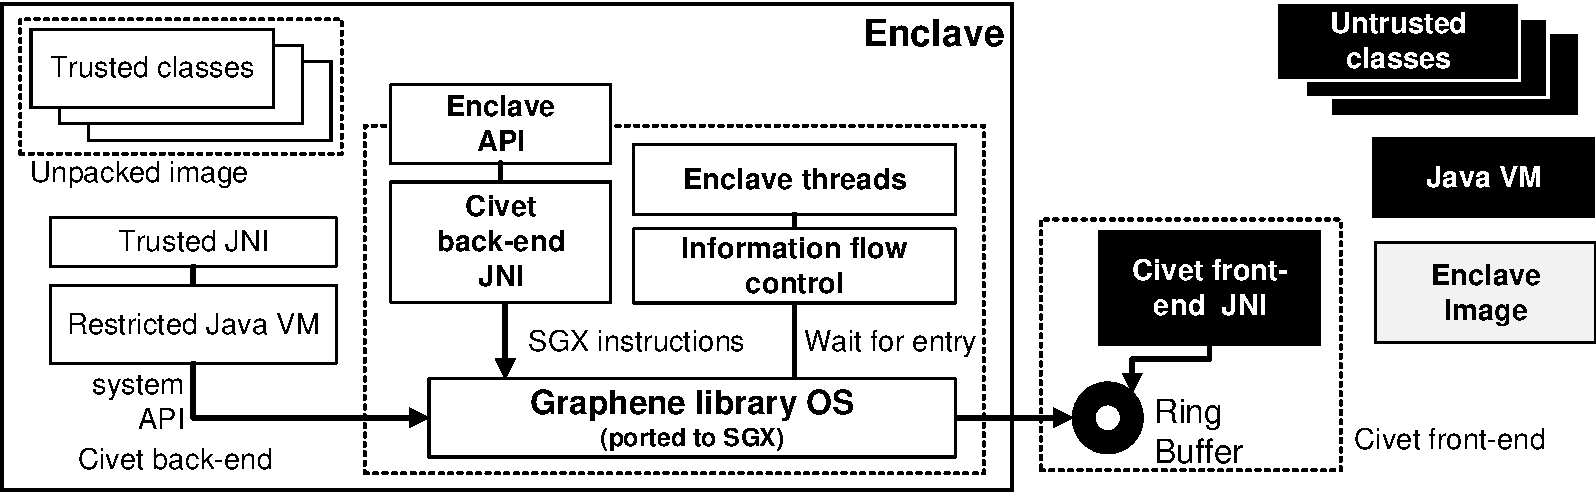
\includegraphics[width=\linewidth]{civet/figures/civet-structure.pdf}
\caption{\systemname{} framework overview.
\systemname{} creates two worlds for an partitioned \java{} application, each with an individual JVM.
The JVM in the enclave is ported using Graphene library OS.
Untrusted classes can invoke methods of trusted classes through proxy objects,
which can transparently access the enclave interface, through serialization
and deserialization over an ring buffer accessed by both untrusted JVM and trusted JVM. }
\label{fig:runtime}
\end{figure}


\subsection{Seamless access to in-enclave objects}
\label{sec:concept:accessing}

For programmer convenience, 
untrusted code can seamlessly call in-enclave objects in \systemname{}.
This is particularly useful when application components are closed-source.
All public methods of trusted, programmer-identified entry classes are entry points for the enclave.
The \systemname{} runtime framework is responsible for generating glue code for entering and exiting
the enclave appropriately, tracking references to objects in the enclave, 
as well as marshalling arguments and return values for in-enclave functions.

%in \systemname{},
%access to in-enclave objects seamless for the untrusted components.
%The rationale behind this design is based on two reasons.
%First, the target of method invocation in \java{} is identified dynamically
%via referencing the object.
%Second, \systemname{} intends to avoid the developers' effort for injecting explicit entry points into the untrusted components,
%especially when the imported \java{} class libraries are close-source.

%% As \systemname{} dynamically determines the enclave entry points in the untrusted components,
%% it avoids the requirement for developers
%% to define the untrusted interface of the enclave.
%% Instead of inquiring manual definition,
%% \systemname{} applies a simple principle to automatically determine the entry points:
%% All public methods of the {\em public} trusted classes can be entry points of the enclave.

In order to reference objects inside the enclave from outside the enclave,
\systemname{} framework uses a byte code generation library --- {\em CGLib}~\citep{cglib} to create untrusted proxies for the in-enclave instances.
CGLib instruments the class that is being proxied,
and redirects the control to a handler 
assigned by \systemname{} upon any method invocation on the proxy.
The proxy then triggers enclave entry to run the trusted method.



%% When untrusted code calls a public method of a trusted class,
%% \systemname{} transparently identifies 
%% determines enclave entry based on whether the objects accessed is in the enclave or part of the untrusted components.
%% As classes can be replicated inside and outside the enclave,
%% the same method of the same class must trigger different behavior according to the sensitivity of the instances.
%% If the object is instantiated in the untrusted components, the method must be run outside the enclave.
%% If the object is instantiated in the enclave, the method should be trapped,
%% and trigger enclave entry to run the method.
 
In general, supporting classes can be duplicated inside and outside of the enclave.
Calls to a supporting class, such as {\tt String}, from inside of an enclave
go to the in-enclave version, and calls from outside the enclave go to the untrusted version.

An exception is made for entry classes, which are not allowed to be replicated.
Rather, any call to an entry class function is placed inside the enclave.
Thus, constructors and static methods of entry classes also cause enclave entries.
We note that this design point was taken to minimize programmer effort in porting to SGX;
alternatively, we could allow an entry class to be replicated by requiring the programmer to 
explicitly annotate calls to object functions.

The \systemname{} design-time tool creates untrusted proxy classes for all entry classes,
in which all constructors and static methods are redirected to
the \systemname{} front-end, which then enters the enclave.
We chose this approach because CGLib disallows redirecting 
constructors and static methods, as this can introduce ambiguity in
the invocation target when all classes are in the same JVM.

%% If the method called is a constructor or static method,
%% the affected object is no longer an instance,
%% but the class itself.
%% To allow seamless invocation of the method,
%% it causes ambiguity for the affiliation of the class, if the class is replicated in both partitions.
%% Therefore, \systemname{} restricts the invocation of constructors or static methods
%% to only the entry classes,
%% and disallows replicating the entry classes
%% in the untrusted components.
%% In addition, if the constructor of an entry class is called upon the constructor of its untrusted subclass,
%% the instantiation will be rejected by \systemname{}.

%% \paragraph{Interception of in-enclave objects.}
%% To seamlessly trigger the enclave entry upon method invocation,
%% \systemname{} intercepts the instances or classes that belong to the isolated components.
%% To intercept non-static method of in-enclave instances,
%% \systemname{} uses {\em CGLib} \fixme{cite} to create proxies of the in-enclave instances.
%% CGLib instruments the class that is being proxied,
%% and redirect the control to a handler assigned by \systemname{} upon any method invocation on the proxy.
%% The handler then triggers enclave entry to run the isolated method.

%% \systemname{} uses a different mechanism of interception for constructors and static methods,
%% because CGLib disallows redirecting constructors and static method
%% due to the ambiguity of invocation targets.
%% Instead, \systemname{} uses the design-time tool to create a dummy classes for all the entry classes,
%% in which all constructors and static methods are redirected to
%% the \systemname{} front-end.
%% Because we disallow replication of entry classes
%% in the untrusted components,
%% loading the dummy classes does not affect functionalities of the application. 

\paragraph{Passing arguments into the enclave.}
When a method triggers enclave entry, the arguments of the method have to be passed into the enclave for the invocation.
\systemname{} always copy the arguments into the enclave,
by serializing the arguments into byte streams,
copying the byte streams into the enclave memory,
and then de-serializing into objects.
By coping arguments into the enclave,
\systemname{} ensures execution of trusted code does not inadvertently leave the enclave.
If the code invokes a method on one of the arguments,
the in-enclave copy of the class is used on an in-enclave instantiation of the object.
Upon de-serialization, the arguments are also automatically type-checked,
thus avoiding the risk of memory corruption.

\paragraph{Returning objects.}
Once the triggered method finishes execution in the enclave,
it may return an object or literal back to the untrusted calling function.
In general, objects are returned similarly to passing input arguments---by serializing the object to a byte stream and returning the bytes.
%Technically, returning objects is the same as passing arguments, and only take serialization and de-serialization.

In order to ensure confidentiality of sensitive data, \systemname{} takes additional care to check
whether a returned object creates an unexpected control flow.
At enclave exit, \systemname{} only allows an object to be returned if it is not tainted with any secret data,
in which case the object is serialized and passed back to the caller.
Section~\ref{sec:security} details our information flow tracking mechanism.

In cases where the object is tainted and an instance of a trusted class,
\systemname{} instead creates a reference in the enclave (to prevent garbage collection of the object internally),
and returns an opaque reference type, that causes the untrusted \systemname{} runtime to create a proxy out of the enclave.
This policy applies to all constructors.
If a proxy object is garbage collected, the destructor calls into the enclave to release the reference on the 
corresponding object in the enclave.
The \systemname{} untrusted runtime is responsible for translating any proxy objects passed as arguments to the enclave into opaque pointers,
which the in-enclave runtime then translates to local object references.

In the case of a tainted literal, we encrypt the plaintext return value concatenated with a nonce, using a temporary key, and return the ciphertext.
This encrypted literal can then be passed to subsequent enclave calls, where the value is decrypted as part of deserialization.

%% However, unconditionally allowing returning objects may become a threat to the information confidentiality of the enclave,
%% because the object may contain part of the enclave secrets due to the information flow.
%% \systemname{} only allows returning objects
%% that are not tainted by the information flow from any secrets. More details about determining the taintedness of the objects are discussed in section~\ref{sec:security}.

%% Based on the taintedness of the objects, \systemname{} has different policies and mechanisms of returning the objects to the caller,
%% to maintain both information confidentiality and progress of the application.
%% The policies are described as follows:

%% \begin{compactitem}
%% \item {\bf the object is not tainted}: serialize and pass the object to the caller.
%% \item {\bf the object is tainted, and is instance of an isolated class}: 
%% create a proxy and intercept future invocation.
%% The policy commonly applies to all constructors.
%% \item {\bf the object is tainted, and is a literal}:
%% automatically encrypt the literal with a default key.
%% \end{compactitem}


%\paragraph{Secure entry and exit of the enclave}
%The \sgx{} hardware ensures that the enclave only has fixed number of entry points (exactly one location where the execution starts, but multiple pre-defined locations that the execution can jump to). 
%The untrusted components must be forbidden to jump to random code in the enclave.
%Moreover, if the isolated component want to exit the enclave,
%it must explicit call the exit instruction ({\tt EEXIT}) to make sure
%the control flow won't be manipulated to leave the enclave.

%\systemname{} models this guarantees by exporting all the public methods of the isolated classes
%(including constructors, static and non-static methods) as the entry points or untrusted interfaces.
%When the untrusted component calls a constructor or static method of an isolated class,
%the execution inside the enclave is triggered,
%either to instantiate the class or perform other operations.
%If a proxy of an isolated instance is returned to the untrusted components,
%the untrusted components can keep it or pass it around.
%As soon as any untrusted components call one of the public methods on the proxy, the execution re-enter the enclave and start the isolated execution.

%Exporting public methods as the entry points or the untrusted interface
%is assumed to be reasonably secure in \systemname{}.
%First, only for the entry classes (the top-most classes of the enclave),
%the constructors or static method will be exported.
%Because developers have expressed that these classes are the ones that interact with the untrusted classes, it is safe to allow the untrusted components to calls these methods and trigger execution in the enclave.
%Second, even if the public non-static methods can be called
%upon isolated classes, the untrusted components can only call upon the proxies,
%which are essentially returned values from the previous method calls.
%Without the proxy, the untrusted components can never call the public methods
%on random instances in the enclave, if the instances are never returned to the untrusted components.


\subsection{Remote Attestation and Provisioning}
\label{sec:concept:others}

\paragraph{Generating attestation reports.}
A feature of \sgx{} hardware is the ability to generate an attestation report for a remote entity,
demonstrating the integrity of the enclave code at launch time.
%The \sgx{} hardware provides the feature of generating a attestation report to prove the integrity of the isolated execution to a remote entity.
\systemname{} provides helper API for developers to access these features,
with convenience and extended trust.
For attestation, \systemname{} generates a report that contains a list of classes loaded inside the enclave, with their measurements.
The report is attached with the attestation generated and signed by \sgx{}, but processed by Graphene.
The \sgx{}-generated attestation contains both
the enclave measurement (proving integrity of Graphene) and
the measurement verified by Graphene (proving integrity of other binaries and files).


%% \fixmedp{Huh?  Really?}
%% The attestation report contains the enclave measurement
%% and is signed using a key derived
%% from the measurements of both sides of attesters,
%% so the remote entity can verify it by retrieving the same key
%% (both attesters must be running in \sgx{} enclaves).

Note that \systemname{} also includes
the dynamic loading state in the attestation report.
%A stronger guarantee provided by \systemname{} than \sgx{}
%is to present the dynamic loading state in the attestation report.
The attestation generated by \sgx{} only contains
the initial state of the enclave, and does not record changes within the executable code
after the enclave starts. 
In both cases, the remote entity is trusting the initially loaded binary
to not dynamically load code that could compromise the enclave;
however, \systemname{} can offer a more precise accounting of the state of the enclave 
at the time a report is generated.

\fixmedp{For future work, would be cool to have some non-editable record of what is added to the enclave, so a corrupted enclave cannot hide the equivalent of a rootkit}

%% As a result, the entity that
%% verifies the attestation report has to blindly trust the initial code
%% in the enclave does not dynamically load any vulnerable code.  
%% The attestation report generated by \systemname{}
%% reflects the latest state of class loading,
%% allowing the trusted entity to audit the execution of enclaves.

% providing a class called {\tt Enclave}, with the APIs that service attestation and provisioning requests.
%The {\tt Enclave} APIs are wrapper to the low-level semantics required by the \sgx{} hardware,such as exchanging the attestations with remote hosts and verifying them, or 
%securing the channels after attesting the other side of communication.
%Because the works are completely hidden beneath the APIs,
%the developers are spared from all the cryptographic details during the process of attestation and provisioning.

\paragraph{Secure provisioning.}
\systemname{} provides an API that transparently validates a connection to a remote host to load
sensitive classes or secret data.
%to be used for secure provisioning.
To use this API, both sides of the connection
must be running in enclaves created by \systemname{}.
The API performs key exchange algorithm (e.g., Diffie-Hellman) on the connection,
secure the connection with encryption,
and authenticate the connection by exchanging the attestation reports.
\systemname{} provides convenient helper functions for developers to create a trusted path
for provisioning sensitive data to a remote enclave.
%Developers can use this API to design any provisioning scheme, without implementing the details of building the trusted path.


\section{Hardening \sgx{} at Enclave Boundary using Information Flow Control in \java{} }
\label{sec:security}

\systemname{} % models the high-level security guarantees and features
%of the \sgx{} hardware in the \java{} language,
allows \java{} developers to directly utilize the security features of \sgx{}, such as isolation from an untrusted hypervisor, % execution, code integrity, etc,
in combination with language-level features that make the code in the enclave more robust.
% safety and advanced protections in \java{}.
%By bridging the gap between language and hardware protections,
%\systemname{} creates opportunities to combine \sgx{} hardware protections
%and security benefits given by \java{} as a managed language.
%In this section, we discussed the opportunities we explore to harden \sgx{} protection with the usage of \java{} language.

%\fixmedp{Honestly, a lot of this is getting pretty repetitive.  I would probably hoist the argument for Java into the motivational text and not bother repeating it here.}

%\subsection{Benefits from the usage of \java{} Language}

%We note that \java{} has several features that can reduce or eliminate
%common vulnerabilities.
%Memory corruption bugs are constant threats to applications
%implemented in C or C++ languages,
%but \java{} applications naturally defend against these vulnerabilities.
%\java{} is immune from memory corruption bugs, such as heap and buffer overflows.
%Several security enhancements come naturally with running \java{} classes
%in the enclave. \java{} applications are known to be immune to memory corruption bugs such as buffer or heap overflow.
%Type casting in \java{} is checked against the type of the target object.
%applications, \java{} perform strict type-checking on the objects to be casted.
%Type-checking prevents corruption of object either in the isolated components,
%or when receiving arguments from the untrusted interfaces.
%Similarly, 
%Similar as the memory corruption bugs,
%Because \java{} is memory safe, it is immune to known control flow attacks, such as return-oriented programming,
%where control flow is manipulated by unsafe writes to return pointers on the stack or function pointers in objects.
%applications implemented in C or C++ languages inevitably face the risk of ROP (return-oriented programming) attacks,
%where attackers can manipulate the control flow by corrupting the applications' stacks or heaps.
%Since \java{} classes can defend against memory corruption,
%attacks cannot manipulate the control flow by overriding the return pointers or function pointers.

%We do assume that the JVM and JNI code are free from memory corruption and control flow attacks.
%Proving a JVM implementation correct is beyond the scope, although similar 
%efforts have been made previously to prove a language runtime correct~\citep{yang10safe}.
%In the case of JNI, we would discourage developers from using JNI code in enclaves if at all possible.

%% Note that although memory corruption bugs and control flows attacks are forbidden in \java{} classes,
%% these vulnerabilities can still exist in the \java{} VM and JNI.
%% In \systemname{} we assume \java{} VM and JNI must be fully trusted,
%% and we leave it as a future work to secure these components.

%% dp: Meh.  prolix
%% For isolated components in the enclaves, memory corruption bugs and control flow attacks are just as dangerous as for other applications.
%% Because the isolated components are fully trusted by the CPU,
%% they can access any memory that are set to proper permissions, including the memory outside the enclaves.
%% Even if a vulnerable component is exploited to copy all the enclave secret out of the enclaves, no hardware solution can effectively stop the exploitation.
%% Even though isolated components cannot directly jump out of the enclave,
%% control flow attack can still manipulate the components to jump to certain locations internally and perform malicious operations. 
%% Therefore, preventing memory corruption bugs and control flow attacks
%% can be a strong reason for application developers
%% to choose \java{} language instead of C/C++ to implement the isolated components.

%\fixmedp{This whole subsection is already covered above.  Commenting}
\begin{comment}
\subsection{Reducing the enclave TCB}

%A \java{} applications often yield a huge TCB, including the \java{} VM,
%JNI and supporting classes that come in bulk.
%For example, a \java{} applications executed by \jvm{}
%will load the \java{} VM binaries up to 40MB \fixme{find out actual numbers}. The classes in the standard \java{} VM libraries such as {\tt rt.jar} includes more than 18,000 classes, and the size of the package is more than 30MB.
%On the other hand, the actual classes needed by an application from {\tt rt.jar}
%can be as less as 1,000 classes.
%Majority of the classes provided from {\tt rt.jar},
%--- even though they may never be loaded into the enclave ---
%still remains in the TCB.

Having unnecessary binaries and classes in the TCB of the enclave
can aggravate the risk of being attacks.
First of all, the huge amount of code loaded into the enclave
increase the opportunity of having gadgets that can be exploited in ROP attacks,  
which can still happen in the \java{} VM or JNI.
Even though most of the \java{} classes have static footprint of their supporting classes,
many of them still dynamically load classes, such as directly calling the class loader, or specifying providers to the \java{} cryptography framework.
Having huge TCB as \java{} classes in the enclave still intensify
the risk of attacks, even though \java{} classes are immune to control flow attacks. 

\systemname{} largely reduce the supporting classes that can be loaded into the enclave,
by partitioning out the necessary classes from all the libraries in the developers' class paths, into the enclave image.
When the enclave is created, the \java{} VM will not load any existing libraries such as {\tt rt.jar} from the host system,
but instead only search classes in the signed enclave image.
Minimizing the supporting classes that can be loaded into the enclave
guarantees that all the classes that are included in the TCB
are actually required by the isolated components,
and come from a trusted source such as the developers' execution environment. 

Note that we do not partition the JNI within the \java{} VM binaries.
We assume partitioning out the JNI functions that are required by the isolated classes
is fully feasible with some manageable efforts.
Moreover, the \java{} classes can be potentially partitioned at a smaller granularity than the whole classes, such as the methods and fields, which can even further reduce the TCB.
We leave these potential improvements as future works. 
\end{comment}

%\subsection{Information Flow Control at Enclave Boundary}
%Problem of not just leaking secrets but also tainted info
As an example of higher-level, language-based analysis, we implemented information flow tracking
in \systemname{}.
A common usage of enclaves is to protect sensitive data, such as an encryption key;
thus, a common concern is that this sensitive data not be inadvertently returned because of an error or exploit within the enclave code.
In general, we chose a design point that minimizes programmer effort; to adopt information flow tracking, we
do require the programmer to specify secret data classes and declassify objects to be released as is from the enclave.

\begin{figure}[t!]
	\centering
	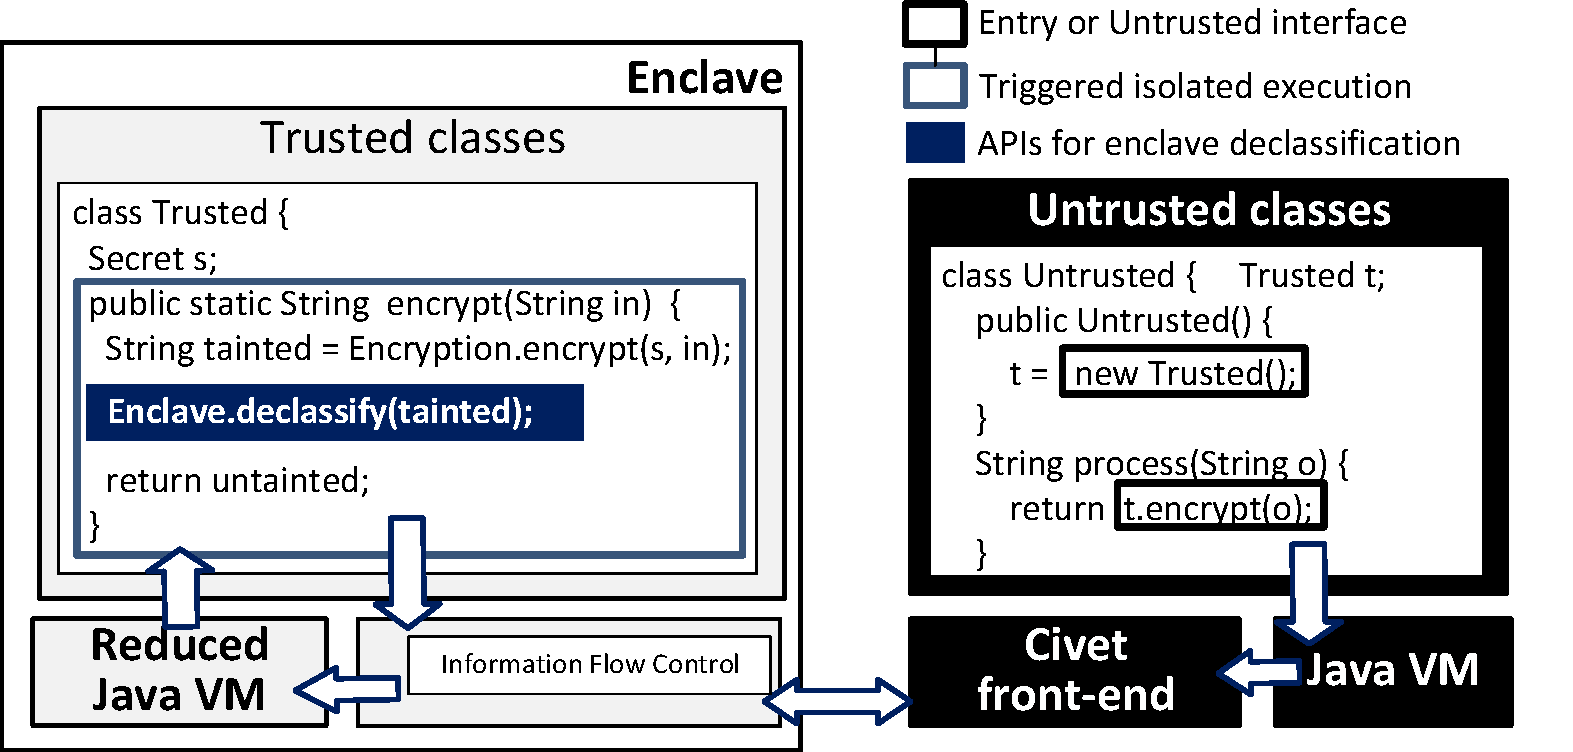
\includegraphics[width=0.9\linewidth]{civet/figures/declassify.pdf}
	\footnotesize
	\caption{How \systemname{} provides a declassifier API to declassify sensitive  data.
		When the untrusted class ({\tt Untrusted}) from Figure ~\ref{fig:synthesis} now calls the {\tt encrypt} method of a trusted class ({\tt Trusted}),
		\systemname{} automatically calls the {\tt encrypt} method inside enclave, and pass the {\tt String} parameter.
		Before returning the result, the trusted class has to use the {\tt declassify} to remove the taint of {\tt tainted} variable that is tainted by the {\tt encrypt} method of class {\tt Encryptor} because of the tainted secret variable {\tt s}.
	}
	\label{fig:declassify}
\end{figure}

%Because the code running in enclave has access to complete address space, including the trusted as well as untrusted memory regions, it is easy for the trusted code to inadvertently undermine \sgx{} protection by writing secret information in the untrusted region. Further, leaking any information derived from or related to the secret may be used by the untrusted code to guess the value of secret information. For example, even in the presence of memory protection, sandboxing and virtualization, it is possible to recover the secret key used by crypto algorithms~\citep{kocher1996timing,osvik2006cache,weiss2012cache, zhang2012cross}. So, to ascertain the secrecy of the sensitive data, no information derived from the secret should exit enclave in plaintext.

%We use JAVA tool phosphor source and sink to taint provisioned data and control leakage
%\systemname{} leverages extensive research on information flow tracking and control in \java{} to harden the \sgx{} security. 

In the enclave, we implement source-to-sink taint tracking, using the open-source Phosphor library~\citep{phosphor}.
%\fixmedp{check this}
The programmer manually selects the classes containing secret data that take secret input from a remotely-provisioned source.
This taint is propagated to any new variables that result from explicit or implicit flows from a secret object.
The only way to remove taint from an object is to pass the object through a \systemname{} declassifier API,
which returns an untainted copy of the object.

%\fixmedp{Would be nice to have a simple example class with a label and declassifier in a figure, if space and time allow}

\systemname{} enforces the policy that only untained data may be returned from an enclave.
If tainted data is being returned, the system transparently encrypts the data and removes its taint before letting the data leave the enclave.
In the cases where a developer wants to return references to sensitive data, \systemname{} instead returns an opaque reference or, in the case of a literal, encrypts the return value.

%mFor tainted data, the developer may opt to either throw a runtime error, or, by default, to return an encrypted object instead.
%The en

% to taint the secret data when provisioned and propagate the taint to any new data generated as an explicit or implicit result of the secret data. We specify the enclave exit points as targets and enforce the policy that any tainted data must pass through a declassifier, that encrypts the data before egress. We only consider the provisioned data as security sensitive, as the enclave image is only integrity protected.

%Declassifier API: correct usage and scenarios
The \systemname{} {\tt Enclave} class provides a {\tt declassify(Object o)} API that creates an untainted
copy of the object.  In practice, we expect this function to be used in conjunction with tests
on the returned data, or cryptographic functions to protect the data in transit across an untrusted channel.

Continuing our example from Figure~\ref{fig:synthesis}, in Figure~\ref{fig:declassify}, if the {\tt Untrusted} class wants to call the {\tt encrypt} method on the trusted object {\tt t}, \systemname{} front-end transparently passes the argument string {\tt o} to the enclave, and the corresponding {\tt encrypt} method is called in the enclave. The secret {\tt s} is tainted because it was provisioned from remote trusted server as shown in Figure ~\ref{fig:synthesis}. As a result, the call to method {\tt encrypt} of class {\tt Encryptor} taints the encrypted output string {\tt tainted}. If the developer had returned this {\tt tainted} variable, the \systemname{} information flow tracking would re-encrypt the ciphertext, and thus make the return value useless for the {\tt Untrusted} class. However, as the developer wants to return the ciphertext as is, she can declassify the {\tt tainted} string by passing it through the declassifier API to get an untainted version of the same object. Such untainted objects can be released from the enclave without further encryption.

%to let the application developer explicitly indicate that the argument object does not contain any secret information, and is safe to leave the enclave as is. For instance, if the enclave code encrypts a blob of data using the tainted secret provisioned key, the information flow will taint the encrypted data. However, because the encrypted data is safe to exit enclave if a perfectly secure encryption algorithm is used, the developer can explicitly mark the encrypted data as declassified. We note that the developers need to be extra careful while declassifying objects to inadvertently leaking secret information.

%Dealing with confidential code
In order to protect the confidentiality of sensitive code,
\systemname{} also allows classes themselves to be tainted.
\systemname{} enforces a policy that any data returned from sensitive code is tainted, and the developer needs to explicitly declassify tainted output data to mitigate
concerns around reverse-engineering the code based on brute-force probing of its outputs.
Of course, the binary code itself is also not allowed to be copied out of the enclave.

% expose it to the untrusted world.
%The {\em code confidentiality} property of \systemname{} loads and executes encrypted classes from remote hosts to protect secret algorithm. We consider this provisioned code as equally security sensitive as provisioned data. ~

%\begin{table*}[t!b!]
\centering
  \begin{tabular}{p{0.05in} >{\raggedright\arraybackslash}p{2.05in} >{\raggedright\arraybackslash}p{4.4in}}
  \toprule
  \multicolumn{2}{l}{\it Security guarantees or features} & {\it The modeling approach applied by \sysname{}} \\
  \midrule
  \midrule
  \multicolumn{3}{l}{\bf Natively provided by the \sgx{} hardware (including the SDK):} \\
  \midrule
  & Isolating security-sensitive components &
  Asking developers to identify multi-level sensitivity, by marking the {\em entry classes}. Complete separation between isolated and untrusted classes.
  \\
  \midrule
  & Secure entry / exit of enclaves &
  Exporting public methods of isolated classes. Arguments are type-checked.
  \\
  \midrule
  & Integrity of the execution environment & 
  Packaging all supporting classes into a signed JAR.
  \\
  \midrule
  & Attestation \& secure provisioning & 
  Providing class {\tt Enclave}, to create secure channels and exchange attestation.
  \\
  \midrule
  \midrule
  \multicolumn{3}{l}{\bf Improvement from combining of \java{} language and the \sgx{} hardware protection:} \\
  \midrule
  & Memory safety \& control flow integrity &
  Naturally provided by \java{} language.
  \\
  \midrule
  & Reducing the enclave TCB &
  Automated partitioning based on class dependencies.
  \\
  \midrule
  & Preventing information flow leakage &
  Tracking information flow in trusted classes, only allow releasing the information if not tainted or declassified by developers.
  \\
  \midrule
  & Code confidentiality & Dynamically loading provisioned classes.
  \\
  \end{tabular}
  
\footnotesize
\caption{
The approaches applied by \sysname{} to model the security guarantees and features of the \sgx{} hardware, and to enhance the security by combining language and hardware protections.
}
\label{tab:features}
\end{table*}

